\chapter{Modelling Ensemble Interaction}\label{chap:mp_network}

\section{Introduction}

% TODO: revisit introduction and discussion and make sure we use the word "style"

Jazz ensemble performances involve intricate processes of coordination among the musicians involved. Through collective improvisation, performers exchange musical ideas, negotiate their roles in the ensemble, and strive to understand each other's intentions in the performance. In particular, jazz musicians display unique (and genre-specific) approaches to embodied musical timing, variously referred to as their ``feel'', ``swing'', ``pocket'', ``time'' \citep[][, also Chapter \ref{chap:rhythm_rsos}]{Berliner1994}, and they must align their timing with their partners' in order to maintain a coherent performance \citep{Doffman2014}. 

Group jazz improvisation thereby exemplifies a particular kind of joint action in which coordination is achieved through multi-level interactive alignment, the process by which the participants in a joint activity come to understand aspects of their shared world in the same way as each other \citep{Garrod2004}. In this respect, jazz improvisation has often been compared to spontaneous spoken conversation \citep{Kello2017, Monson1996}, where alignment towards shared conceptualisations of space and time can also occur between participants. Moreover, the ways in which different ensembles perform together can also be considered to represent a kind of group ``style'' \citep{Hagberg2017}.

In the previous chapter, we saw that there was actually relatively little variation in the interaction strategies adopted by different jazz trios, as modelled using a process of linear phase correction (Figure~\ref{fig:rsos_pianist_networks}). However, one possibility we suggested is simply that musicians operate on ``autopilot'' when performing in idealised (real-time, face-to-face) conditions \citep[see][]{Jacoby2021}. When groups of musicians are prevented from establishing exact rhythmic synchrony, it is possible that they may adopt a more diverse range of strategies. These strategies, in turn, may then reveal interesting aspects of their performance style that we were unable to study in Chapters~\ref{chap:jtd_tismir}--\ref{chap:rhythm_rsos}.

A real-world scenario where exact rhythmic synchrony is impossible can be found when musical performances occur over vast distances, including via the internet. Whenever a sound is transferred over a network, a temporal delay --- known as latency --- is introduced between when it was first produced and when it is received, resulting from the time required to convert sound waves to digital packets and transmit them over a network. While some form of delay is present even when music is performed face-to-face, owing to the time taken for sound to transmit in air, the latency present in networked performances is often several orders of magnitude greater \citep{Chafe2010}. In addition, transmission errors and network congestion can cause fluctuation in packet arrival time, and this variability --- known as jitter --- can cause further instability in (or even the momentary loss of) the output signal during networked performances.

We use variable delay as an experimental manipulation, as it poses significant challenges for successfully coordinating joint action in various forms of time-dependent communication. This includes spoken conversation \citep{Aagaard2022, Boland2022} and interactive music-making \citep{Chafe2010, Chew2005, Rottondi2015}. Network latency impedes the alignment of temporal models and prevents the extreme rhythmic synchrony that is typical of ensemble playing. Networked performances are typically associated with decreased ratings of performance quality and reduced connectedness with co-performers, compared with face-to-face music-making \citep{Bartlette2006, Monache2019, Olmos2009}. Moreover, unlike speech interaction, in musical performance action and interaction are generally organised around a continuous temporally periodic pulse \citep{London2012}, which is highly susceptible to disruption by latency and jitter. Network latency starts to cause problems for interactive musical performances at approximately 28 milliseconds of one-way delay \citep{Chafe2010}; the threshold for negotiating spoken conversations online without difficulty seems to be much higher, at 500 ms \citep{Holub2007}.

Prior research has focussed on optimising networking infrastructure to improve the fluidity and coherence of remote musical performance. This includes the development of low-latency, low-jitter platforms, such as JackTrip \citep{Caceres2010} and LOLA \citep[LOw LAtency audio-visual streaming system,][]{Drioli2013}, that intend to offer the networked ensemble an experience as close as possible to that of playing in the same room as each other. Strategies used by these systems include data buffering, where incoming data packets are stored by the application before being released at regular intervals to ensure consistency in the output signal. But while these technological advances can minimise the presence of a time-lag to performers, latency can never be eliminated completely. A networked ensemble must, therefore, find some way of coordinating their joint action that accommodates this delay in the process.

In this chapter, we consider the relative optimality of strategies for coordinating group musical improvisation, with all the reliance on periodicity and the tight temporal coordination of action that this process entails. In previous work, coordination in face-to-face performances has typically been modelled as a function of one performer's adaptation to any deviations from expected isochrony in another's playing (phase correction or ``coupling'': see \citealp{Jacoby2021}, \citealp{Timmers2014}, \citealp{Wing2014}; see also \citealp{Demos2023}, for a recent review, and Section~\ref{sec:rsos_interaction_features} for a discussion with relation to \GLS{JTD}). In networked performances, one hypothesis is that all players in an ensemble should try hard to listen to each other and couple together, which could result in mutual and symmetrical adaptation to timing variability \citep{Nowicki2013}. An alternative hypothesis is that successful networked interaction requires a degree of asymmetry in the distribution of roles within a musical ensemble: one performer ignores the delayed feedback, while their partner(s) attempt to match and adapt to them \citep{Carot2009}. Participants in prior studies have mentioned adopting either these or similar strategies to accommodate latency during networked performances \citep[e.g.,][]{Bartlette2006}, but the question of which might be optimal has not been systematically explored. 

To address this issue, we conducted a series of experiments where five duos of professional jazz drummers and pianists improvise together over a simulated network. This network introduces delay and jitter of a magnitude up to and including that present on Zoom, a telecommunications platform commonly used in remote interaction and teleconferencing. To evaluate the relative optimality of their coordination strategies, we use a battery of objective and subjective metrics as indicators of the overall success of these performances. We collect data from both MIDI recordings and evaluations provided by the musicians and a secondary sample of naive listeners we recruited via an online listening study. 

We begin our analysis by outlining the results from co-present (i.e., non-delayed) conditions, before then considering how the presence of latency and jitter affects these baselines. Next, we use a combination of linear causal modelling and participant self-reports to characterise the individual coordination strategies and performance style of each duo. Finally, we evaluate the relative optimality of these strategies by conducting computer simulations.

\section{Methods}\label{sec:mp_methods}

\subsection{Participants}	

Ten adult men with a median age of 24 ($SD = 5$, $\text{range} = [21, 36]$) participated in the study. All participants had at least three years of professional experience on either piano or drum kit, held an undergraduate (or higher) degree in music performance, and were fluent English speakers. This combination of instruments was selected as they constitute two-thirds of the ``rhythm section'' in jazz: due to our experimental manipulations requiring real-time MIDI input (see Section~\ref{sec:mp_testbed}), we were unable to accommodate acoustic bass in the ensemble. Participants were recruited from within the author's network of performance contacts and were all professional or semi-professional musicians based in London, UK. Several are internationally renowned, with releases on major record labels and performances in high-profile concert venues and festivals. All individuals who were approached for inclusion participated in and completed the study, with the experiments being conducted between April--July 2022.

Participants were grouped into five duos, each consisting of one pianist and one drummer, with no participant performing in more than one duo. The two musicians in duo 3 had never played together before (but were aware of each other), while the remaining pairs reported performing with together during the past year. However, none of the participants had any prior experience of networked performance with their duo partner before the present experiment. 

This sample size was deemed appropriate because we treated each participant (and duo) as an independent entity, extensively characterising their individual coordination strategy over many performances, rather than focussing on group averages across the entire sample. This approach is typical for psychological studies of advanced musical performance where ensemble roles and interpretative strategies are both highly specialised and individualised, and may depend on pre-existing relationships within a particular participant-group \citep[e.g.,][]{Jacoby2021, Wing2014, Pras2017, Bantula2016, Chang2017}.

The experiment was approved by the Ethics Review Subcommittee at the Faculty of Music, University of Cambridge, UK (reference: 21-22-163). All participants provided written informed consent, including consent for the release of their data in anonymised form and for it to be made available to other researchers. Participants were paid for their time and travel according to the rates specified by the UK Musicians' Union.\footnote{\url{https://musiciansunion.org.uk/rates}}

\subsection{Testbed Configuration}\label{sec:mp_testbed}

\begin{figure}[]
  \centering
  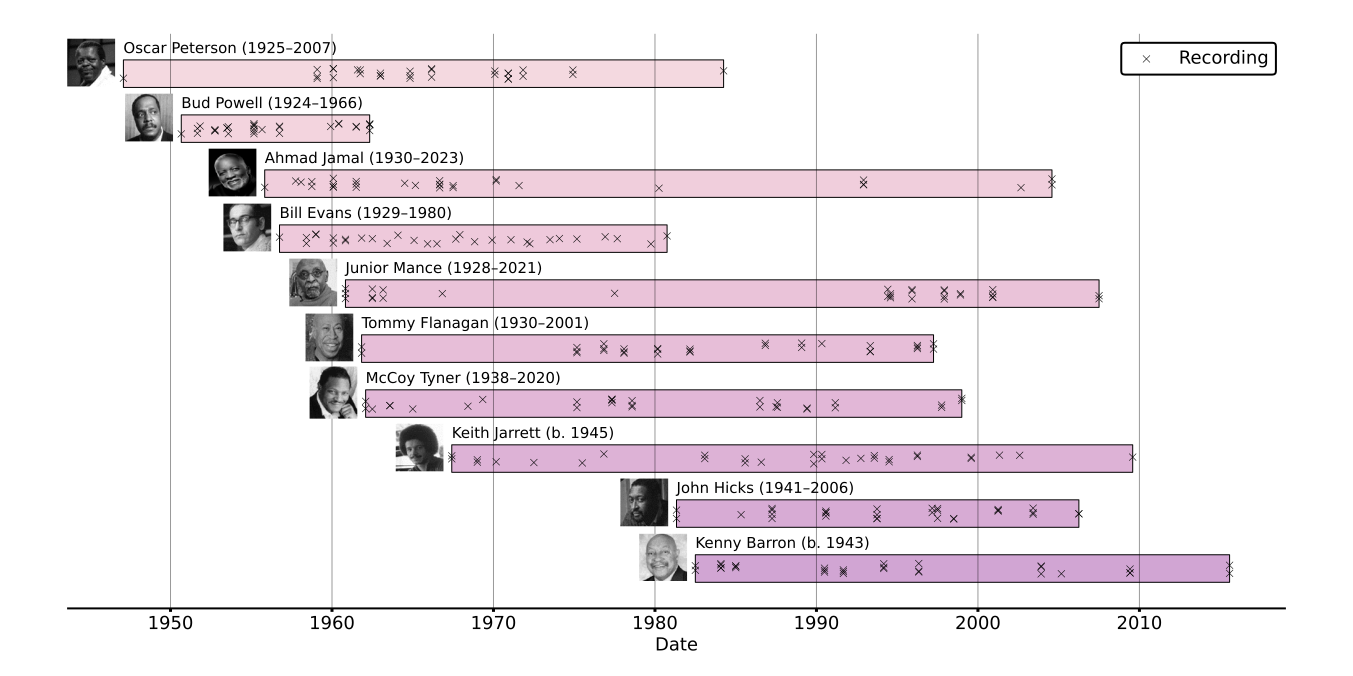
\includegraphics[width=1.0\textwidth]{figures/mp_network/figure_1.png}
  \caption[Configuration for network latency testbed.]{Configuration for network latency testbed. The top row of panels shows (a) the procedure used to measure network latency over Zoom Meetings and (b) the resulting 90-second latency and jitter time-series profile. The bottom row shows (c) a diagram of the testbed layout and (d) how this looked within the experiment room, for pianist and drummer.}
\label{fig:mp_testbed_configuration}
\end{figure}

We designed a novel testbed for the experiment, shown in Figure~\ref{fig:mp_testbed_configuration}. First, we generated a representative measurement of network latency and jitter by connecting two computers on the same network to a virtual call on a popular telecommunications platform (Zoom). Then, we positioned a metronome (playing at 80 quarter note beats per minute) next to one computer, so that an echo could be heard from the speakers of the other computer as each pulse was transmitted (Figure~\ref{fig:mp_testbed_configuration}a). We recorded audio of this process for 90 seconds and derived the variable round-trip latency between pulse and echo by applying the onset detection algorithm (using the ``spectral flux'' method: see Section~\ref{sec:jtd_alternate_methods}) contained in the \texttt{librosa} (version \texttt{0.8.1}) Python library \citep{McFee2015}, to the recording. Network latency was generally stable around a median peak-to-peak delay of 192 ms ($SD = 17.7$, $\text{range} = [181, 293]$ ms), with occasional spikes caused by jitter (Figure~\ref{fig:mp_testbed_configuration}b). 

\begin{figure}[]
  \centering
  \includesvg[width=1.0\textwidth]{figures/mp_network/figure_s1}
  \caption[Additional network latency tests.]{Additional network latency tests. Each column of plots shows the variable latency time experienced during a 90-second teleconferencing call on Zoom Meetings, created following the procedures used in Figure~\ref{fig:mp_testbed_configuration}a. The left-most column shows the network latency measurements used in the present study, given also in Figure~\ref{fig:mp_testbed_configuration}b. The remaining columns show results from identical tests in three different locations. In each column of plots, the $y$-axis shows the latency time between initial metronome beat and echo, normalised such that the minimum delay time is 0 ms. The $x$-axis shows either the duration of the call (line plot), or the density function (histogram).}
\label{fig:mp_additional_network_tests}
\end{figure}

We conducted identical tests in three different locations, using different network configurations. These were: (1) a recording studio, with both devices connected wirelessly to an institutional network; (2) the same studio, with one device connected to the institutional network and the other wirelessly to a mobile cellular network; (3) a home office, with one device connected via Ethernet to a commercial router and the other to a mobile cellular network. These produced broadly similar results (Figure~\ref{fig:mp_additional_network_tests}), which suggests that our measurements resemble the typical experience of using this platform for telecommunication.

The testbed was designed to apply these measurements to a performance in a controlled fashion --- simulating a network, not directly implementing one \citep[as in][]{Rottondi2015}. In the experiment room (an acoustically isolated recording studio), both participants sat apart from each other, with barriers placed to prevent direct visual contact (Figure \ref{fig:mp_testbed_configuration}c). Separate video and MIDI streams were captured of their performances, using an electronic keyboard (\texttt{Nord Electro 6D-73}), drum kit (\texttt{Roland TD-27KV}), and two computer webcams (\texttt{Logitech Brio 4K Pro}). Video was captured at a resolution of $1920 \ \times \ 1080$ px and a rate of 30 frames per second. These signals were then transmitted to a computer server via USB connection and a 32-channel MIDI interface (\texttt{M-Audio MIDISPORT $2 \ \times \ 2$}).

We implemented the software components of our testbed in the Python programming language. Variable latency was applied to each musical track using the digital audio workstation \texttt{REAPER} (version \texttt{6.46}).\footnote{\url{https://www.reaper.fm/}} Communication with the Python back-end was handled using the \texttt{ReaPy} bindings (version \texttt{0.10.0}).\footnote{\url{https://github.com/RomeoDespres/reapy}} Each time a note was played, the corresponding latency was determined by looking up the current value in the latency time series (Figure~\ref{fig:mp_testbed_configuration}), and the playback of that note was then delayed by that amount. Delay times were resampled from the latency time series at periodic intervals of 750 ms to replicate the metronome speed of the original test. Latency was applied to each video track in the same manner, using the \texttt{OpenCV} \citep{Bradski2000} computer vision library in Python (version \texttt{4.5.5.64}).

The server then stored both the incoming (live) and outgoing (delayed) signals for later analysis before presenting them to participants. MIDI signals were first transcoded to audio using high-quality virtual instrument libraries (\texttt{Addictive Keys} and \texttt{Steven Slate Drums}), and then routed back at a rate of 44.1 kHz through a 16-bit digital-to-analogue converter. Video was shown on individual 27-inch computer monitors in front of each participant. Participants heard and saw delayed audio and video from their partner's performance, alongside non-manipulated audio of their own playing. They did not see video of themselves, due to the additional computational demand this would introduce and the likelihood that this would obstruct the view of their partner and their instrument (Figure~\ref{fig:mp_testbed_configuration}d). Participants wore closed-back headphones to eliminate the acoustic sound of their partner's instrument.

During testing, we found that the inherent delay added by our testbed signal path to the incoming MIDI signal was 4 ms for the keyboard and 3 ms for the drums. This is significantly lower than the inherent audio latency reported in previous studies \citep[e.g.,][]{Olmos2009, Rottondi2015} and likely stems from our use of MIDI, rather than audio. This value is not included in the reported results, as it is likely perceptually sub-threshold \citep{Grant2004}. The inherent delay for the incoming video signals was substantially greater, at 33 ms (i.e., one frame). This is likely due to the greater computational demands involved in the real-time processing of video compared to audio. Rather than applying additional latency to the MIDI to compensate for this, we instead allowed both audio and video to be unsynchronised, which is common during networked performance and teleconferencing \citep{Rottondi2016}.

\subsection{Experimental Design}

We selected a ``twelve-bar blues'' structure in the key of $\text{B}\flat$ as the musical stimulus for the experiment. This simple, repetitive form is pervasive in jazz and popular music \citep{Katz2017} and was immediately familiar to all participants, all of whom chose to perform it from memory and without the aid of a musical score. Performances lasted 90 seconds, the same duration as our measured latency time series, meaning that the total number of repeats of the blues form was dictated by the tempo established by the musicians. Before the experiment began, participants completed three warm-up performances without any latency and at a variety of tempi, allowing them to practise together in the testbed environment. The remaining performances comprised the experimental session and were characterised by differing amounts of latency and jitter.

We operationalised latency by transposing the original latency time series $d$ (Figure~\ref{fig:mp_testbed_configuration}b) so that $\text{min}(d) \in \{23, 45, 90, 180\}$ ms, not including the inherent delay introduced by the testbed. This latter value (180 ms) was within the upper limit of latency times tested in prior research and was essentially equivalent to the minimum delay we had originally measured on Zoom (181 ms); the other values tested were the integer quotients resulting from the successive division of 180. We manipulated jitter by keeping the minimum latency value as set above but scaling the deviations from this minimum value by either 1.0x (no change from original variation measured on Zoom), 0.5x, or 0.0x (no jitter, consistent/``flat'' delay). The procedure used to transform the original latency time series $d$ to the latency time series $d'$, with minimum latency time $L$ and jitter scaling $J$, can be written as:

\begin{align}\label{eq:mp_latency}
d'^N_1=\biggl(J\biggl(d_i-\text{min}(d^N_1)\biggr)+L\biggr)^N_1
\end{align}

\begin{figure}[]
  \centering
  \includesvg[width=1.0\textwidth]{figures/mp_network/figure_2}
  \caption[Experimental conditions for network latency study.]{Experimental conditions for network latency study. The thirteen conditions tested in the experiment were derived from the transformation of the measurements in Figure~\ref{fig:mp_testbed_configuration}b. The rows indicate minimum latency values between 0 and 180 ms, with jitter scaling shown by the colour of each line. The left column shows the raw latency timings over the 90-second duration of each performance. The right column displays the standard deviation of latency values obtained over a sliding window of four seconds, which we use in the partial correlation analysis of timing variance shown in Figure~\ref{fig:mp_partial_correlations}}
\label{fig:mp_experimental_conditions}
\end{figure}

We also test a final control condition where we do not apply latency or jitter to the signals, beyond that introduced by the testbed (i.e., $L = 0, \ J = 0$). These thirteen conditions were presented to duos in a randomised order across two successive sessions with a break of one hour in between, with each condition appearing once in every session. Figure~\ref{fig:mp_experimental_conditions} shows the transformations of the latency time series that were used in each condition.

\subsection{Experimental Procedure}\label{sec:mp_experimental_procedure}

Before each performance began, participants heard sixteen quarter-note pulses from a synthesised metronome over their headphones at a moderate tempo of 120 quarter-note beats per minute, which is a typical speed for a medium tempo jazz blues. The first of each group of four pulses was played at a higher pitch and greater dynamic level than the others to clarify the meter as four quarter-note beats per measure. The total duration of this count-in was eight seconds.

\begin{figure}[]
  \centering
  \includesvg[width=1.0\textwidth]{figures/mp_network/figure_s2c}
  \caption[MIDI note distribution.]{MIDI note distribution. Both ``instruments'' show the frequency of MIDI note placement across all performances in the dataset; the darker the colour, the more often that particular drum or piano note was played by participants. Values are scaled so that the most frequently played note has a normalised value of 1. Note that the rims of the snare, rack, and floor toms were tracked independently of the centre of these drums, and are coloured accordingly. Additionally, the ride cymbal is separated into bell (centre) and bow (edge), and the hi-hat into cymbal (struck with the stick) and pedal (operated with the foot). Only the four octaves of the piano keyboard that were used most frequently are shown here.}
\label{fig:mp_instrument_heatmaps}
\end{figure}

Participants were then instructed to improvise together over the blues form while maintaining both the tempo and meter established by the metronome pulses by playing continuous quarter notes. More specifically, the pianist was asked to play either a ``walking bass'' or ``stride'' accompaniment pattern, and the drummer was asked to ``play time'' on their hi-hat, ride cymbal, and bass kick drum in a swing style. In Figure~\ref{fig:mp_instrument_heatmaps}, we analyse the frequency of MIDI note distribution across the total range of each instrument to demonstrate that performances broadly conformed to the given brief. 

Participants were not made explicitly aware of the presence of latency and jitter. Instead, they were told that the feedback they would receive from their partner would change during the experiment, and that they should interact with them as they otherwise would during a ``real'' performance. To that end, we encouraged participants to improvise light musical embellishments while following their assigned brief, provided that this did not disrupt their ability to maintain the underlying quarter-note pulse.

Each performance lasted for 90 seconds before participants were instructed to stop. Recording was then maintained for several seconds to prevent notes from being cut off if they occurred shortly before the 90-second point; the following analyses only consider the first 90 seconds of a performance, however.

\begin{figure}[]
  \centering
  \includesvg[width=1.0\textwidth]{figures/mp_network/figure_s3}
  \caption[Test-retest reliability from performance questionnaire.]{Test-retest reliability from performance questionnaire. Each bar shows the inter-rater (i.e. between both the pianist and drummer in a duo) and test-retest (i.e. between matched scores for each condition across both sessions of the experiment) reliability of the questions presented to performers in the experiment. The $x$-axis shows each question, with values of Pearson's $r$ on the $y$-axis. Bar colouring corresponds to duo numbers. Asterisks above a bar indicate the significance of the correlation coefficient, $^* \ p < .05, \ ^{**} \ p < .01, \ ^{***} \ p < .001$.}
\label{fig:mp_performer_questionnaire_test_retest}
\end{figure}

After each performance, participants were asked to complete a questionnaire evaluating their subjective experience of that performance in terms of: (1) the quality of the interaction with their duo partner; (2) the ease of coordination with their partner and; (3) the overall success of the performance. These questions were administered using the \texttt{Qualtrics} online survey platform and are similar to those used in an earlier study of improvised duo interaction by \citet{Setzler2020}. Participants provided responses to each question using integers from one to nine inclusive, with lower scores corresponding to negative and higher scores to positive evaluations. We show measurements of test-retest reliability in Figure~\ref{fig:mp_performer_questionnaire_test_retest}. Participants were also invited to optionally comment on a performance in free text.

\subsection{Listener Evaluations}\label{sec:mp_listener_evaluations}

As we could not assume that our participants would provide an unbiased assessment of the quality of their own performance \citep{Pras2017, Schober2014}, we also obtained equivalent evaluations from listeners recruited online via the \texttt{Prolific} platform. This experiment was implemented in the \texttt{PsyNet} (version \texttt{10.2.0}) software package \citep{Harrison2020}, which enables large-scale perceptual studies to be conducted online through a web browser interface, and is also used in Section \ref{sec:gen_subjective_evaluation}. Participants were required to: (1) be at least 18 years old, (2) use headphones, (3) be in a quiet environment where they can clearly see their computer screen, and (4) use an up-to-date Google Chrome browser. 

A pre-screening listening task that asked participants to discern differences in the volume of three synthesised sounds \citep{Woods2017} was presented at the start of the experiment to exclude participants who were not listening attentively over headphones. Successful participants were then shown recordings (audio and video, with latency and jitter applied to both participants) of the first 45 seconds of 15 random performances, and were asked to rate how successful they thought it was along a nine-point scale. Of the three questions initially answered by our performers, only the performance success question was used in this experiment as it was most likely to be comprehensible to listeners, who were not required to have any prior experience of listening to jazz. Participants were told only that the performances were taking place over the internet, and were not informed about the explicit amount of latency or jitter used. 

\begin{figure}[]
  \centering
  \includesvg[width=1.0\textwidth]{figures/mp_network/figure_s4b}
  \caption[Demographic information from subjective listening test.]{Demographic information from subjective listening test. Each bar plot shows the proportion of responses to every demographic question presented to each participant in the listening evaluation test.}
\label{fig:mp_listener_demographics}
\end{figure}

\begin{figure}[]
  \centering
  \includesvg[width=1.0\textwidth]{figures/mp_network/figure_s4c}
  \caption[Distribution of results from subjective listening test.]{Distribution of results from subjective listening test. Each plot shows 95\% confidence intervals obtained from bootstrapping (with $N = 10,000$ replicates) over the listener-reported success scores ($x$-axis) obtained for each condition ($y$-axis).}
\label{fig:mp_listener_results_distribution}
\end{figure}

Eighty-eight adults (44 women, 42 men, 2 non-binary) with a median age of 38 ($SD = 14$, $\text{range} = [18, 75]$) participated in the study, excluding those who failed pre-screening tasks. For full demographic details, including information on participants' musical background, see Figure~\ref{fig:mp_listener_demographics}. We calculated this sample size by determining the approximate number of participants required to obtain 10 ratings of each of the 130 performances in the dataset, assuming each participant rated 15 performances. In reality, not all performances received the full number of ratings, due to attrition caused by network time-outs or participants otherwise ending the study early: 31 (23.8\%) performances were rated by 9 participants, and 6 performances (4.6\%) were rated by 8 participants. Responses were generally consistent across different participants rating the same performance (Figure~\ref{fig:mp_listener_results_distribution}).

The experiment was approved by the Ethics Review Subcommittee at the Faculty of Music, University of Cambridge, UK (reference: 21-22-163), and all participants provided written informed consent. Participants were compensated at a GBP £10/hour rate, according to the amount of the experiment they completed; thus, if a participant failed a pre-screening task or left the study early, they were still paid for the proportion of the task that they had completed.

\subsection{Beat Extraction}

\begin{figure}[]
  \centering
  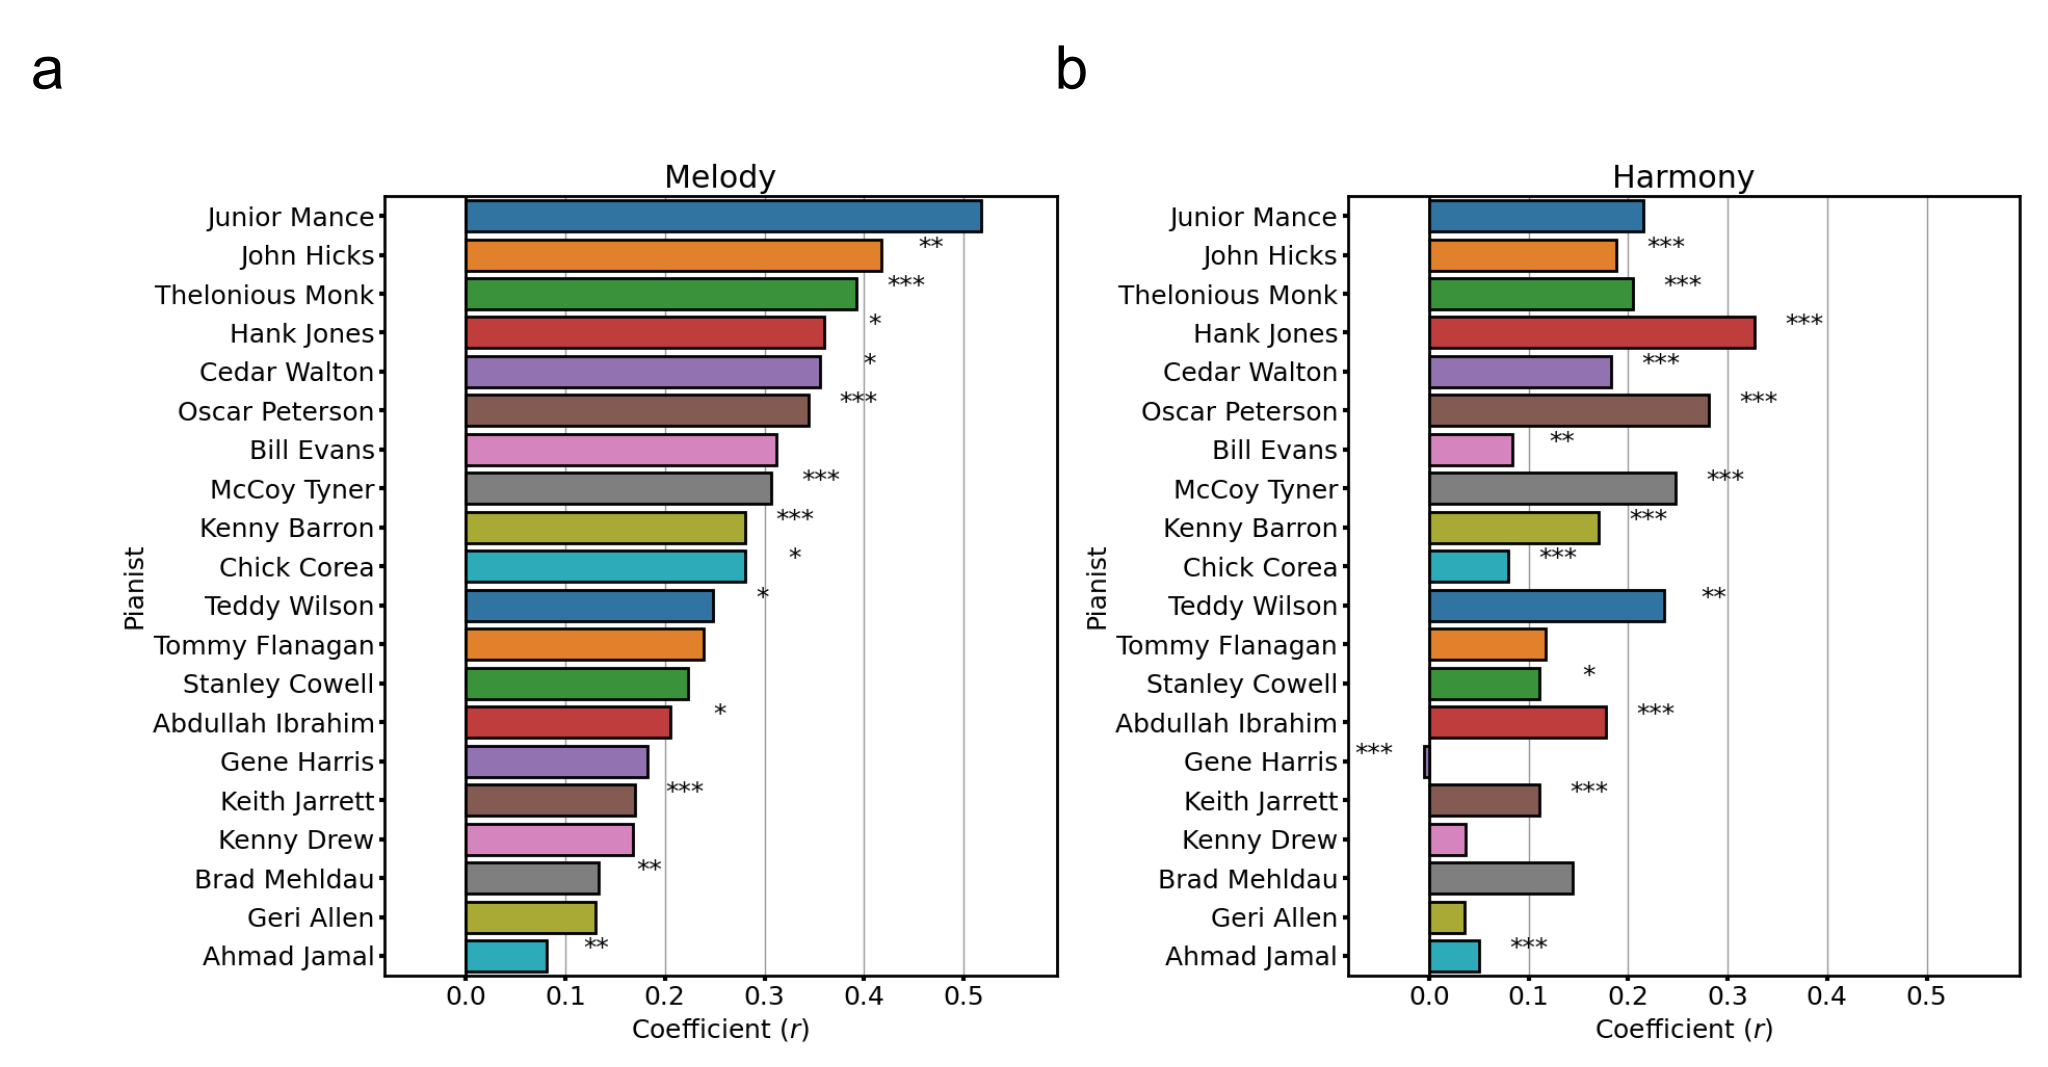
\includegraphics[width=1.0\textwidth]{figures/mp_network/figure_3.png}
  \caption[Beat extraction procedure.]{Beat extraction procedure. (a) shows notation from a hypothetical performance where linear interpolation would be applied. The note annotated with an exclamation point in the upper stave has been ``pushed'' before its expected position as the first beat of the next bar. The lower stave shows the performance after interpolation, with this note aligned midway between the quarter notes immediately before and after it (the inter-beat interval between which is given by $y$). (b) shows the total number of beats contributed by each participant to the final dataset, after filtering and nearest-neighbour matching. The hatched segment of each bar shows the proportion of beats by that performer that required interpolation, with the exact number of beats given above the bar.}
\label{fig:mp_beat_extraction_procedure}
\end{figure}

For each of the 130 performances in the dataset, we extracted the position of the MIDI onsets corresponding to each quarter-note beat by manually removing any improvised embellishments from the non-manipulated (live) recordings. In a minority of performances, the regular quarter-note pulse was occasionally disrupted, either due to mistakes made by participants or due to syncopated anticipation (``pushing'') of the quarter-note beat ahead of its expected metrical position \citep{Berliner1994}. Missing (or anticipated) quarter notes were detected through inspection of the MIDI data, using the video recordings of a performance for reference as necessary. We then realigned these notes into their expected position through linear interpolation between those beats occurring immediately before and after (Figure~\ref{fig:mp_beat_extraction_procedure}a).

Repeat notes (where one musical event was incorrectly registered as two or more MIDI notes) were filtered from performances in the dataset by discarding any quarter-note beats where a preceding beat occurred less than 250 ms before. These repeat notes may have inadvertently occurred due to a performer pressing a piano key or hitting a drum pad several times in rapid succession. We chose this threshold as it is half the duration of quarter-note inter-beat intervals at the reference tempo provided to participants (500 ms); we deemed it unlikely that participants would have accelerated to more than twice this initial tempo.

We then used a nearest-neighbour algorithm to match each quarter-note beat from one performer with the closest equivalent beat played by their partner, with the addition of the latency applied by the testbed at that moment in time. In cases where two consecutive beats by one participant could conceivably be matched with the same beat by their partner, we consider only the pair with the minimum temporal distance. This accounts for instances where a performer may have inserted an additional quarter note into their performance to realign with their partner \citep{Berliner1994}; e.g., ``[I] popped an extra beat in a middle fill'' (drummer, duo 1), ``I added an extra beat towards the end of the recording to get back on [beats] 2 and 4'' (pianist, duo 3).

The raw dataset consists of 46,640 quarter-note beats, 2.7\% of which required linear interpolation. Filtering repeated MIDI notes from the performances results in a loss of 0.4\% of the raw data, with the nearest-neighbour matching incurring a further loss of 4.0\%. The final dataset comprises 44,605 matched quarter-note beats, extracted from four hours of MIDI performances (Figure~\ref{fig:mp_beat_extraction_procedure}b).

\subsection{Feature Extraction}

We extract three objective measures of coordination success from the matched quarter-note beats dataset: (1) tempo slope, which captures any systematic digression from the reference tempo; (2) asynchrony, the extent to which both performers remain ``in time'' with each other; and (3) timing irregularity, the local variability of quarter-note inter-beat intervals. We also extract two subjective measures of performance success: (1) the ratings provided by the musicians themselves, and (2) the average rating given by participants in our online perceptual study. 

A formal definition of tempo slope is given in Section~\ref{sec:jtd_tempo} and Equation \eqref{eq:tempo_slope}. We calculate this metric individually for each performer and then average across the ensemble, to reflect the fact that one musician's tempo would not feasibly be independent of their partner's when both are attempting to play together (see Section~\ref{sec:rsos_tempo_features}).

We define asynchrony as the root-mean-square of the temporal distance between all matched beat pairs articulating the same metrical position played by both musicians \citep{Clayton2020}, including the latency applied by the testbed to both beats. Thus, the asynchrony $A$ for performer $i$ to performer $j$ with latency $d'$ can be written as
\begin{align}\label{eq:mp_asynchrony}
A_{i,j} = \sqrt{\frac{1}{N} \sum\limits_{k=1}^{N} \biggl((t^i_k+d'^i_k) - (t^j_k+d'^j_k)\biggr)^2}
\end{align}
where $t_k$ is the timestamp of quarter-note beat $k$ and $N$ is the total number of beats in the performance. We obtain a single asynchrony value from each performance, which represents the experience of a hypothetical listener joined to the same virtual ``call'' as our duo (i.e., the perspective of the participants in our online study). Note that, as all performances began at the same reference tempo, we do not need to express asynchrony proportionally to the duration of a quarter-note beat as we did earlier in Section~\ref{sec:jtd_synchrony}.

We define timing irregularity as the relative temporal instability of a performance, as characterised by the moment-to-moment variability in quarter-note beat durations. We compute this metric by: sliding an overlapping window of four seconds duration (equivalent to two measures at the reference tempo and meter) over both performers' quarter-note inter-beat intervals (i.e., seconds 0--4, 1--5, and so on), taking the standard deviation of inter-beat intervals within the window, and calculating the median of all standard deviation values. We use windowed statistics due to their increased robustness to trends and patterns in time series analysis. If the tempo or a performance slowed down or sped up, for instance, the series of inter-beat interval durations would be non-stationary and the mean interval duration would change over time.\footnote{Note that a similar feature was extracted in the analysis presented in Section~\ref{sec:rsos_tempo_features}, with the bounds of the window based on the bar annotations contained in \GLS{JTD}, as opposed to ``clock time''.} We obtain two values for timing irregularity for every performance: i.e., one for each musician.

We define performer-reported success as the responses given by participants to the question ``how successful was the performance?'' with a rating of 1 indicating an ``extremely unsuccessful'' performance and 9 an ``extremely successful'' one. This question showed the best test-retest and inter-rater reliability of the three asked to performers (Figure~\ref{fig:mp_performer_questionnaire_test_retest}). However, levels of inter-performer agreement are still not especially high: averaging values of Pearson's $r$ obtained from correlating the scores given by pianists and drummers in every duo, $\text{mean}(r) = .40$ ($SD = .24$, $\text{range} = [.17, .73]$). This suggests only moderate agreement between performers on average. Disagreements of this kind are common in group musical improvisation, however, where performers rarely share the same understanding of what exactly unfolded \citep{Pras2017, Schober2014}, and should not be taken to indicate any inherent lack of reliability in the data.

We define listener-reported success as the mean rating given by listeners to a single performance: note that individual ratings of the same performance were generally consistent ($\text{mean}(SD) = 1.64$; see also Figure~\ref{fig:mp_listener_results_distribution}). Average levels of listener-pianist and listener-drummer agreement are broadly equivalent with the levels of pianist-drummer agreement given above: when values of the correlation coefficient $r$ are averaged across all duos, listener-pianist $\text{mean}(r) = .33$ ($SD = .39$, $\text{range} = [-.32, .72]$), listener-drummer $\text{mean}(r) = .40$ ($SD = .15$, $\text{range} = [.19, .56]$). Our musicians did not hold a privileged understanding of the success of their own performances \citep{Schober2014}: they agreed with listeners to an equivalent degree that they agreed with each other.

\subsubsection{Data Availability}\label{sec:mp_data_availability}

We make all data and research materials (including MIDI and video recordings) created as part of the experiments described in this chapter available under a permissive licence on a trusted third-party repository.\footnote{\url{https://doi.org/10.5281/zenodo.7773824}} The code for the analyses reported in this chapter is also publicly accessible,\footnote{\url{https://github.com/HuwCheston/Jazz-Jitter-Analysis}} as is our testbed \footnote{\url{https://github.com/HuwCheston/AV-Manip}} and perceptual study\footnote{\url{https://github.com/HuwCheston/2023-duo-success-analysis}} software. All participants consented to the public, non-commercial release of their data under these conditions. Anonymised transcripts of the free-text responses given by participants are also provided in Appendix~\ref{chap:mp_appendix}. All statistical analyses and models reported in this chapter are implemented using the \texttt{SciPy} (version \texttt{1.9.0}, \citealp{Virtanen2020}) and \texttt{statsmodels} (version \texttt{0.13.5}, \citealp{Seabold2010}) Python libraries.

\section{Results}

\subsection{Baseline Measurements for Non-Delayed Performances}

\begin{figure}[]
  \centering
  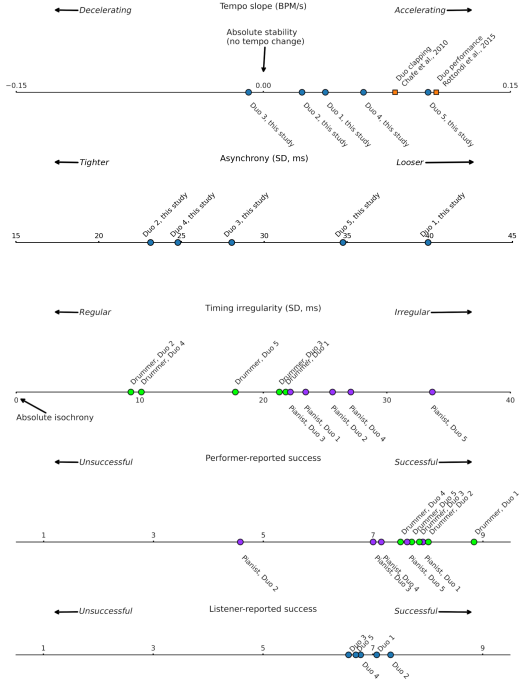
\includegraphics[width=1.0\textwidth]{figures/mp_network/figure_4.png}
  \caption[Results from baseline (no latency) performances.]{Results from baseline (no latency) performances. Number lines showing baseline values obtained for tempo slope, asynchrony, timing irregularity, performer- and listener-reported success. Values are averaged for both repeats of the ``no latency'' condition by a duo. Note that integer values are randomly displaced horizontally for visual clarity.}
\label{fig:mp_baseline_results}
\end{figure}

\begin{figure}[]
  \centering
  \includesvg[width=1.0\textwidth]{figures/mp_network/figure_s5}
  \caption[Performance tempo maps from network latency experiment.]{Performance tempo maps from network latency experiment. Time is shown on the $x$-axis and tempo (in quarter-note beats per minute) on the $y$-axis for all 130 performances in the dataset, separated by ensemble (rows) and testbed configuration (columns). The grey dotted line in each plot shows the reference tempo provided to participants before each performance. Both blue and orange lines show moving averages of the performance tempo, using a window of 8 seconds duration (four measures at the reference tempo). The blue lines show performances from the first session of the experiment, and the orange lines performances from the second session.}
\label{fig:mp_performance_tempo_maps}
\end{figure}

In the following discussion, we outline the baseline results obtained from the control condition, when no latency or jitter was applied to the performance (Figure~\ref{fig:mp_baseline_results}). We later use these performances as part of the training data for the generative model described in Chapter \ref{chap:conditioned_gen} (see Table \ref{tab:gen_finetuning_dataset}).

The baseline mean tempo slope for all our duos during the control condition is 0.04 beats-per-minute-per-second (BPM/s) ($SD = 0.03$, $\text{range} = [-0.02, 0.10]$ BPM/s), indicating that the tempo of performances remained stable when no latency was present, though with a slight tendency towards acceleration. In Figure~\ref{fig:mp_baseline_results}, we compare these results with tempo slope coefficients obtained from previous networked performance studies, noting that the behaviour of our duos did not differ from expected standards. In Figure~\ref{fig:mp_performance_tempo_maps}, we show individual ``tempo map'' plots for each performance.

The baseline mean asynchrony for our duos is 33.1 ms ($SD = 7.2$, $\text{range} = [22.5, 48.8]$ ms), which we compare in Figure~\ref{fig:mp_baseline_results} to prior studies of real-time ensemble performance across various musical genres. We note that this value is greater than the asynchrony observed in a prior study of jazz bass and drums synchronisation \citep{Kilchenmann2015}, closer instead to the synchronisation of Cuban salsa or North Indian raga musicians \citep{Clayton2020}. This may be because of the random placement of the control within each experimental session and participants' overall lack of awareness of our manipulations; they could have been primed to adopt particular strategies in non-delayed performances as a result of earlier conditions where latency had been present. For instance, one pianist described how it ``felt slightly more difficult to coordinate, and to be creative'' (pianist, duo 4) during the control in comparison to the previous condition. Another explanation is that the digital environment created by the testbed simply made it harder to play music together effectively versus the face-to-face, co-present conditions used in these reference studies, even without latency and jitter \citep{Doherty-sneddon1997}.

The baseline timing irregularity is 16.1 ms ($SD = 5.8$, $\text{range} = [7.9, 22.1]$ ms) for drummers and 26.4 ms ($SD = 4.5$, $\text{range} = [21.9, 36.7]$ ms) for pianists, which suggests significantly lower variability in the timing of drummers compared to pianists (see also Section~\ref{sec:jtd_tempo}). Note that no participant demonstrated precise temporal isochrony: indeed, anisochronous timing is typically understood to be preferable to ``quantised'' isochrony in music such as jazz \citep[``participatory discrepancies'': here, see][]{Keil1987}.

The baseline mean performer-reported success score is 7.9 ($SD = 0.7$, $\text{range} = [7, 9]$) for drummers and 6.9 ($SD = 1.9$, $\text{range} = [2, 8]$) for pianists, suggesting that real-time performances were regarded as more successful than unsuccessful. Inter-participant agreement was typically higher in their evaluation of the control condition than in the remainder of the experiment, with an absolute difference between pianist and drummer scores of no more than one obtained for nine out of ten control performances.

The baseline mean listener-reported success score is 7.1 ($SD = 0.6$, $\text{range} = [6, 8]$); in Figure~\ref{fig:mp_listener_results_distribution}, we demonstrate that there were no significant differences in mean listener score for performances in the control condition across any duo. These results again indicate that the non-delayed, real-time performances of all duos were consistently regarded by listeners as successful.

\subsubsection{Linear Associations Between Variables}

\begin{figure}[]
  \centering
  \includesvg[width=1.0\textwidth]{figures/mp_network/figure_5}
  \caption[Univariate and bivariate distributions.]{Univariate and bivariate distributions. The histograms on each diagonal show the distribution of the variable plotted in that column/row. The scatter plots below the diagonal show the pair of variables obtained at the intersection of every column and row. Markers represent the score obtained by each duo for all thirteen conditions, averaged across both musicians and sessions of the experiment. The straight red lines show a linear regression model fit between both variables, with error bars denoting 95\% confidence intervals generated via bootstrapping ($N = 10,000$ replicates). Likewise, values above the diagonal denote the coefficient of Pearson's $r$ calculated between the corresponding variable pair, with the font size also indicating the strength of the correlation. Asterisks indicate the significance of the correlation coefficient, $^* \ p < .05, \ ^{**} \ p < .01, \ ^{***} \ p < .001$. Values for the tempo slope variable are given in their absolute (unsigned) form.}
\label{fig:mp_univariate_bivariate_distributions}
\end{figure}

In Figure~\ref{fig:mp_univariate_bivariate_distributions}, we show the pairwise associations between the five performance success variables discussed above. Tempo slope is given in its absolute (unsigned) form to show the relationship between individual metrics and deviations from the reference tempo, regardless of whether this change had occurred via acceleration or deceleration. We observe here that the three objective metrics derived (absolute tempo slope, asynchrony, and timing irregularity) all correlate negatively with both reported success variables --- such that performances that diverged from the reference tempo and displayed lower synchronicity and isochronicity were evaluated less favourably by both participants and listeners. Additionally, tempo slope coefficient and timing irregularity also positively correlate with each other, with a larger magnitude of tempo change associated with more unstable performances.

\begin{figure}[]
  \centering
  \includesvg[width=1.0\textwidth]{figures/mp_network/figure_6}
  \caption[Objective features affecting success evaluations.]{Objective features affecting success evaluations. The panels show standardised regression coefficients ($\beta$) for a mixed-effects model predicting success ratings from musicians and listeners, respectively. Error bars represent 95\% confidence intervals computed by bootstrapping with ($N = 10,000$ replicates). Where an error bar does not cross 0, the effect of that predictor is statistically significant at $p < .05$.}
\label{fig:mp_objective_features_affecting_success}
\end{figure}

To establish the relative importance of the factors involved when evaluating a performance, we fit mixed-effects models predicting performer- and listener-rated success using absolute tempo slope, timing irregularity, and ensemble asynchrony as predictors (Figure~\ref{fig:mp_objective_features_affecting_success}). A random effect (intercepts and slopes) of duo number is included in both models, as we wish to also model group-specific variations in both baseline ratings and the effects of the predictors. The statistical significance of the fixed effects is assessed by bootstrapping over duos ($N = 10,000$ replicates) to produce 95\% confidence intervals. 

For performers, an increase in timing irregularity is the strongest predictor of a subsequent decrease in rating, although all three predictors are significant; for listeners, timing irregularity and asynchrony are both significant predictors of rating decreases (with asynchrony having the stronger effect), while tempo slope is not significant. The amount of variance explained by both the fixed and random effects (conditional $R^2$) is $.762$ for the performer reports and $.856$ for the listener reports. The amount of variance explained by only the fixed effects (marginal $R^2$) is $.483$ for the performer reports and $.735$ for the listener reports. The standard deviation in scores estimated for the random effect of duo is $.970$ for the performer reports and $.520$ for the listener reports. These statistics indicate that the objective metrics effectively summarise the proximal causes of subjectively evaluated performance success. Listeners cared most about whether performers remained stable and synchronised, but not whether they changed tempo, while musicians considered all three factors to be important.

\subsection{Network Latency Impairs Musical Performance}

To evaluate the effect of testbed configuration on the performance of each group, we fit separate linear models to the data obtained for the five duos, using each of our performance success variables as a response measure (i.e., $N = 25$ models total). Latency and jitter are used as predictors in every model and are treated categorically (with the control condition as the reference category), due to the possibility of non-monotonic effects. For models predicting timing irregularity and performer-reported success (i.e., where separate values are obtained individually for both musicians), instrumental role is additionally included as a predictor, with the drummer's performance used as the reference category. 

\begin{figure}[]
  \centering
  \includesvg[width=1.0\textwidth]{figures/mp_network/figure_s6a}
  \caption[Reliability of performance success metrics.]{Reliability of performance success metrics. Each panel shows the test-retest reliability for every performance success metric by comparing values obtained from the first session of the experiment with those from the second. The straight black line corresponds with a simple linear regression, with confidence intervals obtained via bootstrapping ($N = 10,000$ replicates). Integer values corresponding to performer-rated success scores are jittered horizontally and vertically to reduce over-plotting.}
\label{fig:mp_performance_success_reliability}
\end{figure}

\begin{figure}[]
  \centering
  \includesvg[width=1.0\textwidth]{figures/mp_network/figure_s6b}
  \caption[Bias of performance success metrics.]{Bias of performance success metrics. Each plot compares the difference in means for every performance success metric across experimental sessions. The $x$-axis shows the difference in means between sessions, such that a positive value corresponds to larger scores obtained in the second set of the conditions than the first. Error bars show 95\% confidence intervals obtained via bootstrapping ($N = 10,000$ replicates); where a bar does not cross the dotted line, the difference in means between sessions for that combination of performers and metric is significant.}
\label{fig:mp_performance_success_bias}
\end{figure}

We account for our repeated-measures design by averaging the results obtained from a duo for a particular condition across both sessions of the experiment. Values of Pearson's $r$ obtained from the correlation of scores from both sessions of the experiment indicate good to excellent test-retest reliability for each metric (Figure~\ref{fig:mp_performance_success_reliability}): for tempo slope, $r(63) = .66, \ p < .001$, for timing irregularity, $r(63) = .86, \ p < .001$, for asynchrony, $r(63) = .98, \ p < .001$, for performer-reported success, $r(63) = .67, \ p < .001$, and for listener-reported success, $r(63) = .78, \ p < .001$. We also bootstrap the differences in mean scores obtained for each metric across both sessions ($N = 10,000$ replicates). Barring duo 2 demonstrating a significantly greater mean tempo slope coefficient in the second session of the experiment compared with the first (mean difference = 0.03, 95\% CI: $[0.02, 0.04]$), there are otherwise no significant differences (Figure~\ref{fig:mp_performance_success_bias}). These analyses suggest that the behaviour of each duo was consistent across both sessions of the experiment.

The average $R_{adj}^2$ value for our models is .529 when predicting tempo slope ($SD = .529$, $\text{range} = [-.390, .884]$), .985 when predicting asynchrony ($SD = .009$, $\text{range} = [.973, .993]$), .908 when predicting timing irregularity ($SD = .051$, $\text{range} = [.842, .961]$), .717 when predicting performer-reported success ($SD = .175$, $\text{range} = [.407, .820]$), and .885 when predicting listener-reported success ($SD = .062$, $\text{range} = [.821, .971]$). We take this as an indication that testbed configuration and instrumental role alone are generally strong enough predictors to explain a large degree of the variance in each performance success metric, albeit with greater spread of $R_{adj}^2$ values obtained for some metrics than others.

\begin{figure}[]
  \centering
  \includesvg[width=0.9\textwidth]{figures/mp_network/figure_7}
  \caption[Effects of network testbed configuration on performance success variables.]{Effects of network testbed configuration on performance success variables. The bars show regression coefficients from models predicting one of the five performance success variables, with results split by duo. The reference category for each model corresponds to the performance during the control condition (i.e., with no latency or jitter); if values are obtained separately for each instrument for a given variable, the reference category also corresponds to the drummer's performance. Crosses indicate where a particular predictor variable is omitted from that model. Error bars represent 95\% confidence intervals computed by the model; where an error bar does not cross 0, the effect of that category is statistically significant.}
\label{fig:mp_testbed_configuration_on_success}
\end{figure}

\begin{figure}[]
  \centering
  \includesvg[width=1.0\textwidth]{figures/mp_network/figure_s7}
  \caption[Inferential statistics computed across all duos.]{Inferential statistics computed across all duos. The points show the mean value obtained for a given performance success metric, averaged over all performances made using a particular latency or jitter condition. Error bars show 95\% confidence intervals, obtained via bootstrapping over duos ($N = 10,000$ replicates). Where two error bars do not cross, the difference between two latency or jitter values is statistically significant.}
\label{fig:mp_inferential_statistics_across_duos}
\end{figure}

Figure~\ref{fig:mp_testbed_configuration_on_success} plots the coefficients and confidence intervals obtained for every predictor and categorical level in our models, Figure~\ref{fig:mp_inferential_statistics_across_duos} shows inferential statistics for each success metric across every latency and jitter value (averaged over all duos). We organise the following discussion to address in turn the effect of latency, jitter, and instrumental role on performance success.

\subsubsection{Effects of Latency} 

Increases in latency are strongly correlated with increases in ensemble asynchrony, $r(63) = .97, \ p < .001$. This is expected, given how this metric is calculated: see Equation \eqref{eq:mp_asynchrony}. The effect of latency on the remaining metrics is more complex. The lowest amount of latency we tested, 23 ms, predicts significantly reduced ratings of performer-reported success for three duos, but no equivalent changes in any other metric. Above this value, latency has a detrimental effect on many performance features. Both 45 and 90 ms of latency produce significant decreases in tempo slope and increases in timing irregularity for two duos, alongside reductions in performer-reported success for all duos. For listener-reported success values, 45 ms of latency predicts significant decreases in ratings for two duos and 90 ms for all duos. These differences between performer- and listener-reported success at 45 ms latency could suggest a lower tolerance for latency exists when performing versus listening to music. In total, our results replicate many of the ``classic'' findings of earlier networked performance studies, where latency typically contributes to a recursive slowing in the tempo of a performance and reductions in timing regularity and ensemble synchrony, alongside reductions in subjective assessments of performance quality \citep{Bartlette2006, Chafe2010, Monache2019, Rottondi2015}. 

Surprisingly, the maximum amount of latency we tested, 180 ms, is not associated with significant decreases in tempo slope coefficient for any duo. This contradicts the argument made previously by \citet{Chafe2010}, that a linear relationship exists between increases in delay time and decreases in tempo. Instead, this amount of latency is associated with positive tempo slope coefficients for four duos, suggesting that their tempo either accelerated or remained stable. One possible cause of this phenomenon is that, at higher latency values, networked musicians operate more on ``autopilot'', ignoring their partner and focussing solely on the stability of their own performance. For instance, one drummer described the sensation of performing with 180 ms of latency as ``being on parallel tracks'' with their partner, ``rather than being locked in together'' (duo 2). An alternate explanation is that, at extreme amounts of latency, a performer's perspective of the relative phase of their partner's meter inverts. At a tempo of 120 quarter notes per minute, 180 ms of latency is relatively close to the duration of an eighth note (250 ms), and closer still to a triplet eighth note (167 ms). Consequently, this amount of latency means that performers could perceive their partner as playing \emph{ahead} of the next beat, rather than \textit{behind} the previous beat. This could lead to recursive tempo acceleration, as both performers continually rush to catch up with each other. 

The free-text responses given by participants after each performance attest to the effects of latency. Comments range both from acknowledging the changes in performance tempo (``to me, it felt like a constant rallentando that kept failing to land'': drummer, duo 1, ``there was a tendency to rush'': drummer, duo 3) and timing regularity (``when the time isn't settled I have a tendency to tense up'': drummer, duo 2) caused by latency, to annoyance at their inability to interact with their partner successfully (``frustrating to not be able to use body language effectively'': drummer, duo 1), and finally to a dislike of their performance in the testbed environment (``absolute carnage and I think it sounded utterly awful'': pianist, duo 1). It is also worth noting the more positive tone used to describe performances made at 180 ms latency (``everything seemed to align this time'': pianist, duo 1, ``we were on the same page with this one'': pianist, duo 3, ``lots of creative energy'': pianist, duo 4) compared with lower values.

\subsubsection{Effects of Jitter}

\begin{figure}[]
  \centering
  \includesvg[width=1.0\textwidth]{figures/mp_network/figure_s8}
  \caption[Model comparisons using ``backward'' feature elimination.]{Model comparisons using ``backward'' feature elimination. This plot shows averages from five linear regression models predicting one of five performance success metrics, using the data from each duo individually. The $x$-axis shows the combination of predictor variables contained within each model. The $y$-axis corresponds with the amount of variance explained by the model predictors, using the average $R_{adj}^2$. Error bars in both plots show 95\% confidence intervals obtained via bootstrapping over all $R_{adj}^2$ values ($N = 10,000$ replicates).}
\label{fig:mp_model_comparisons}
\end{figure}

While a spike in network latency time caused by jitter inevitably causes large asynchronies in performances at a local scale, at a global scale the jitter conditions we tested seemingly have a much smaller impact on our performance success metrics. The presence of 1.0x jitter predicts significant increases in asynchrony for two duos, increases in timing irregularity for one duo, decreases in performer-reported success for one duo, and decreases in listener-reported success for two duos. The magnitude of these effects, however, is typically much smaller compared with the other predictors. 

We observe a similar trend by systematically removing features from these models and measuring the resulting change in how well it fits the data (i.e., ``backwards'' feature elimination, $\text{mean}(\Delta R_{adj}^2)$: see Figure~\ref{fig:mp_model_comparisons}). Removing jitter as a predictor results in little change to how well each model fits the data obtained for any variable or duo ($\text{mean}(\Delta R_{adj}^2) = 0.01$). In comparison, removing either latency ($\text{mean}(\Delta R_{adj}^2) = -0.69$) or instrumental role ($\text{mean}(\Delta R_{adj}^2) = -0.61$) results in much larger changes.

A complementary way to quantify the effect of jitter is to analyse whether moment-to-moment fluctuations in latency are followed by increased variability in performance timing. To do so, we measure the standard deviation of the quarter-note inter-beat intervals played by a performer and the latency time applied by the testbed across a sliding window of four seconds duration. We then compute partial correlations between these two time series, with latency variability lagged at increasing one-second intervals between 0 and 8 seconds (two bars). To account for any autocorrelation \citep[see][]{Cheston2022}, we control for any prior variation in a performer's timing up to this lag: thus, when computing the partial correlation between timing variability $t$ and latency variability $d$ at lag $k$ seconds, we control for prior timing variability at all lags up to and including lag $k$, except for when $k = 0$ (in which case the correlation is equivalent to Pearson's $r$). 

\begin{figure}[]
  \centering
  \includesvg[width=1.0\textwidth]{figures/mp_network/figure_s9}
  \caption[Partial correlation plots.]{Partial correlation plots. Each column of plots corresponds to one of the three jitter scales tested in the experiment. The $x$-axis shows the degree of lag in seconds applied to rolling measurements of the standard deviation of the latency time series used in the performance (see Figure~\ref{fig:mp_experimental_conditions}, right column) and to prior inter-beat interval variance. The $y$-axis shows values of the coefficient $r$ averaged across all performances in the dataset, irrespective of duo or instrument. Error bars show 95\% confidence intervals of $r$ obtained by bootstrapping ($N = 10,000$ replicates).}
\label{fig:mp_partial_correlations}
\end{figure}

We calculate these partial correlations separately for all performances made using the three jitter values tested in the experiment, regardless of minimum latency (Figure~\ref{fig:mp_partial_correlations}). We observe that, when the 1.0x jitter scaling was used, previous variation in network latency positively correlates with future variation in performance timing. The strongest association between prior increases (or spikes) in latency and future increases in timing variability occurs at a lag of two seconds: averaged across performances by all musicians made with 1.0x jitter, $\text{mean}(r) = .11$ (95\% CI: $[.08, .14]$, obtained via bootstrapping across all obtained values of $r$ with $N = 10,000$ replicates). However, the small magnitude of this correlation suggests that jitter only had a slight impact on performance stability.

Comments by the musicians validate this claim. While they were evidently aware of the presence of jitter (``moments of ride cymbal jolting'': pianist, duo 4, ``noticed the [video] fluctuating'': pianist, duo 5), participants were able to develop strategies to accommodate it. These included inserting or missing beats (``there were several points where we were suddenly playing on different beats to each other, but it was easy to add/drop a beat to come back in time'': drummer, duo 3), cultivating a deeper sense of rhythmic intensity in the performance (``subtle disruptions in the feed were subsumed within the strength of our interaction/groove'': pianist, duo 4), and looking at the video feed (``eye contact and watching the fingers on the [piano] keys helped'': drummer, duo 3). Indeed, one participant even claimed that the disruption caused by jitter had had a positive effect (``disruptions through the feed, but these helped with the flow of the music ... we were able to use [the disruptions] to interact consistently and vibrantly'': pianist, duo 4).

\subsubsection{Effects of Instrumental Role}

Instrumental role significantly predicts differences in timing irregularity for four of five duos, with pianists showing increased variability in beat duration compared with drummers. Instrumental role also predicts changes in performer-reported success for all duos, with pianists associated with higher ratings in three duos and lower ratings in the remaining two. In the case of timing irregularity, pianists may have been less comfortable with the networked conditions (or the procedures of the experiment) than drummers, or alternatively adopted a role in their ensemble that enabled them to perform with more flexible timing (see Section~\ref{sec:jtd_synchrony}). In the case of performer-reported success, it is not uncommon for musicians to develop very different understandings of the same performance \citep{Schober2014}.

\begin{sloppypar}
Removing instrumental role as a predictor of both timing irregularity and performer-reported success results in a substantial effect on $R_{adj}^2$; for timing irregularity, $\text{mean}(\Delta R_{adj}^2) = -0.72$, for performer-reported success, $\text{mean}(\Delta R_{adj}^2) = -0.50$ (see Figure~\ref{fig:mp_model_comparisons}). Vice-versa, removing the testbed condition (i.e., both latency and jitter) has altogether less of an impact on the amount of variance explained when predicting these variables: for timing irregularity, $\text{mean}(\Delta R_{adj}^2) = -0.37$, for performer-reported-success, $\text{mean}(\Delta R_{adj}^2) = -0.35$ (Figure~\ref{fig:mp_model_comparisons}). This implies that variation between participants contributes more to these measures than testbed configuration.
\end{sloppypar}

\subsection{Jazz Ensembles Adopt Diverse Coordination Strategies During Networked Performance}

The members of any musical ensemble coordinate via complex, distributed processes of mutual attending and adaptation \citep{Clayton2020, Jacoby2021, Timmers2014, Wing2014}, which may be referred to by jazz musicians as ``hooking up'', ``grooving'', and ``swinging'' \citep{Berliner1994, Monache2019}. For a group of musicians to remain synchronised, they must adapt to any small deviations from isochrony in each other's performances. When one musician adapts to match variation in another's performance, we can say that they are influenced by --- or ``coupled with'' --- that musician; vice-versa, the absence of coupling implies that one musician does not correct for variability in another's performance, and is thus not influenced by them \citep{Jacoby2021, Konvalinka2010}. In the context of networked music-making, the perception of timing variability in a performance will be affected by any network instability or jitter present in the output signal: a musician does not, therefore, couple with the real-time performance of their partner, but with the delayed feedback they receive from the network \citep{Roman2019}. 

We begin this section by describing the linear phase correction model we employ to model this process, alongside a series of control analyses we conduct to validate it. We then describe the results from applying these models to the performances in our dataset, including evidence suggesting the presence of two distinct coordination strategies employed by the duos.

\subsubsection{Phase Correction Modelling}\label{sec:mp_phase_correction_modelling}

We model the coordination in a networked ensemble using a linear phase correction model \citep{Vorberg1996}, where a performer's upcoming quarter-note inter-beat interval is predicted by both the duration of their prior inter-beat interval and the asynchrony with their partner at the previous quarter note beat \citep{Jacoby2021}. We consider the particular coordination strategy adopted by a networked ensemble equivalent to the complete system of coupling responses established between all combinations of musicians in an ensemble (see Figure~\ref{fig:rsos_pianist_networks}), and hence we create a separate model for each performer in our duos.

\begin{figure}[]
  \centering
  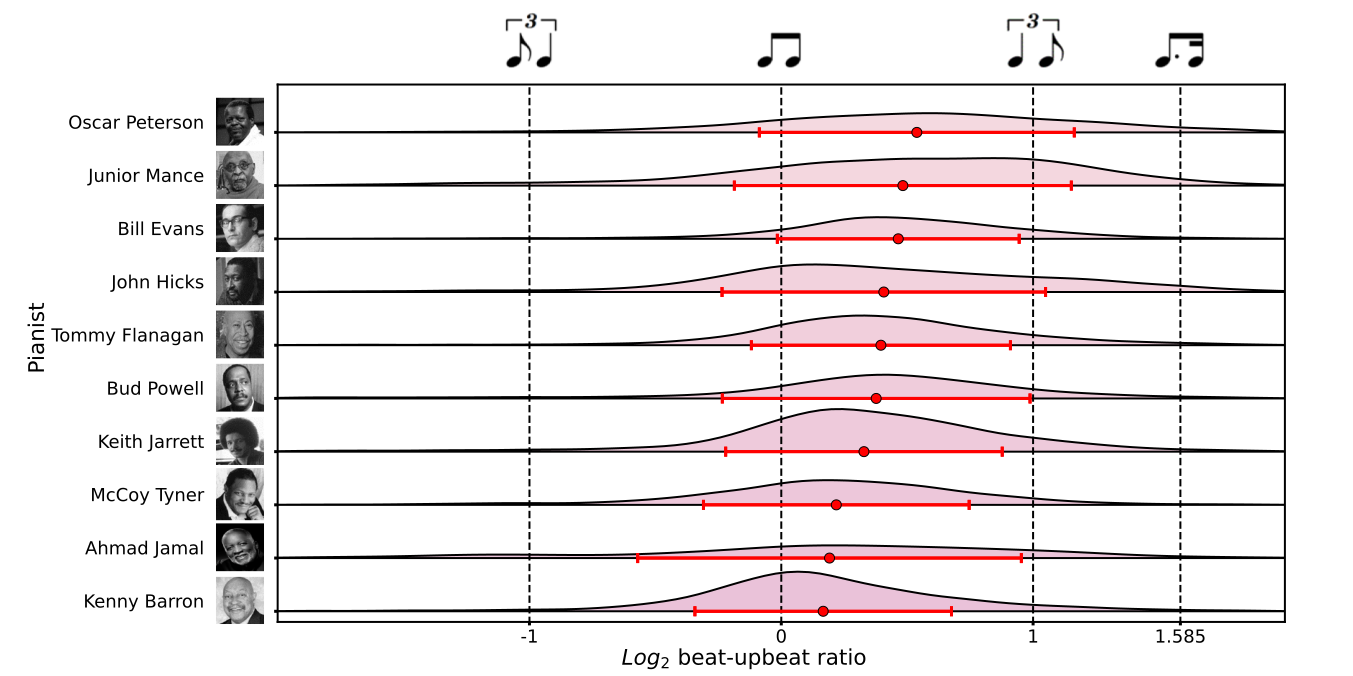
\includegraphics[width=1.0\textwidth]{figures/mp_network/figure_8.png}
  \caption[Measured coupling between the musicians in each duo.]{Measured coupling between the musicians in each duo. (a) is a schematic diagram of the linear phase correction model. Quarter-note beats are given by coloured circles: the circles with dashed borders show the position of beats after latency has been applied, representing when they would have actually been heard by a performer. The vertical grey rectangles indicate the metric grid of quarter notes, while horizontal and diagonal black lines show the inter-beat interval between quarter notes, either from one performer or between performers (asynchrony). The braces indicate the difference between successive inter-beat intervals played by the same musician. (b) depicts the mean coupling coefficient obtained for each participant. (c) shows the mean coupling strength and asymmetry across each duo. Error bars in both (b) and (c) show 95\% confidence intervals of the mean obtained via bootstrapping ($N = 10,000$ replicates). (d) groups the duos by their respective coordination strategy, with the direction and degree of the coupling in each duo given by the colour and thickness of the arrows respectively. Values above each arrow show the mean coupling coefficient, with parentheses indicating standard deviations. Duos are ordered, left-to-right, by average coupling asymmetry across all conditions.}
\label{fig:mp_coupling_model}
\end{figure}

We refer to a single performance by a duo in our dataset as $K$, which can be described as two separate time series comprising sequences of quarter note beat positions $t$ contributed by two musicians, $i$ and $j$. Beat onset positions are measured in seconds from the start of performance, meaning that the performance of performer $i$ in dataset $K$ is given by the sequence 
\begin{align}
K_i = \biggl(t_k^i\biggr)_{k=1}^N,
\end{align}
where $N$ is the index of the final beat in $K$ and $t_1^i > 0$.

For each performer, we obtain the sequence of inter-beat intervals $T$, equivalent to the duration of each quarter note beat that they played. The sequence of inter-beat intervals by performer $i$ is thus written as 
\begin{align}\label{eq:mp_model_timeseries}
\biggl(T^{i,i}_k\biggr)^N_{k=2} &= \biggl(t^i_k - t^i_{k-1}\biggr)^N_{k=2}. 
\end{align}

Note that if the tempo of a performance changes over time, then the mean and variance of $\biggl(T^{i,i}_k\biggr)^N_{k=2}$ will change also, with individual quarter note inter-beat intervals $T^{i,i}$ trending towards smaller or larger values as $k$ increases. To remove any such pattern or trend, we transform the time series in Equation~\eqref{eq:mp_model_timeseries} by taking the signed first difference of inter-beat intervals $T'^{i,i}$, equivalent to the difference in duration of successive quarter notes $T^{i,i}_k$ and $T^{i,i}_{k-1}$. This creates the de-trended time series 
\begin{align}\label{eq:mp_timeseries_detrended}
\biggl(T'^{i,i}_k\biggr)^N_{k=3} &= \biggl(T^{i,i}_k - T^{i,i}_{k-1}\biggr)^N_{k=3},
\end{align}
which is equivalent to
\begin{align}
\biggl(T'^{i,i}_k\biggr)^N_{k=3} &= \biggl((t^i_k - t^i_{k-1}) - (t^i_{k-1} - t^i_{k-2})\biggr)^N_{k=3}.
\end{align}

As described in Section~\ref{sec:mp_methods}, we then use a nearest neighbour algorithm to match every quarter note beat $t_k$ played by performer $i$ with the nearest beat played by their partner $j$. From these matched beats we compute the ``actual'' beat asynchronies of performer $j$ from the perspective of performer $i$ as 
\begin{align}
\biggl(T_k^{i,j}\biggr)_{k=1}^N &= \biggl(t_k^i - t_k^j\biggl)_{k=1}^N. 
\end{align}

We then compute the ``perceived'' beat asynchronies of performer $j$ from the perspective of performer $i$ as 
\begin{align}
\biggl(T'^{i,j}_k\biggr)_{k=1}^N &= \biggl(t_k^i - t_k^j + d^j_k\biggl)_{k=1}^N,
\end{align}
where $d'^j_k$ is the amount of delay applied by the testbed at the point when musician $j$ played beat $k$, and $d'^j_k>0$ for all possible values of $k$ and in all experimental conditions, apart from the control.

We can now write the complete linear phase correction model as 
\begin{align}\label{eq:mp_phase_correction_model}
T'^{i,i}_{k+1} &= \alpha_{i,i} T'^{i,i}_k + \alpha_{i,j} (T^{i,j}_k+d'^j_k) + \alpha_{i,0} + \varepsilon^i_k \ . 
\end{align}
$T'^{i,i}_{k+1}$ is the predicted difference between the durations of the quarter notes by musician $i$ at beats $k + 1$ and $k$, $T'^{i,i}_k$ is the difference between the durations of the two quarter note inter-beat intervals directly preceding $T'^{i,i}_{k+1}$ by musician $i$ (i.e. at beats $k$ and $k - 1$), $T^{i,j}_k$ is the asynchrony between musicians $i$ and $j$ at beat $k$, $d'^j_k$ is the variable delay applied to musician $j$'s performance by the testbed at beat $k$, $\alpha_{i,i}$ is the influence of the previous inter-beat interval difference by musician $i$ on the duration of $i$'s future quarter notes, $\alpha_{i,j}$ is the coupling coefficient reflecting the influence of musician $j$ on future quarter note durations by their partner $i$, $\alpha_{i,0}$ is an intercept term specific to musician $i$, and $\varepsilon^i_k$ is residual noise.

Note that the perspectives of $i$ and $j$ in $K$ are modelled separately; so, rewriting Equation~\eqref{eq:mp_phase_correction_model} to predict the performance of $j$ instead,
\begin{align}\label{eq:mp_phase_correction_model_alt}
T'^{j,j}_{k+1} &= \alpha_{j,j} T'^{j,j}_k + \alpha_{j,i} (T^{j,i}_k+d'^i_k) + \alpha_{j,0} + \varepsilon^j_k \ . 
\end{align}

The mean $R_{adj}^2$ for our model across all performances is .487 ($SD = .128$, $\text{range} = [.094, .742]$), meaning that it typically captures about half of the total variability in differenced inter-beat interval durations during a performance. This is broadly comparable to the range of values given in Section~\ref{sec:rsos_interaction_features}.

\subsubsection{Control Analyses}\label{sec:mp_phase_correction_control_analyses}

We further verify the consistency and reliability of phase correction as a model of synchronisation behaviour by conducting a series of four control analyses.

Our first control analysis investigates the reliability of our model by computing Pearson's $r$ between coupling coefficients $\alpha_{i,j}$ and $\alpha_{j,i}$ obtained from the first and second sessions of the experiment. We find a strong positive correlation between coupling in both sessions, $r(63) = .81, \ p < .001$, suggesting that the synchronisation behaviours used by our participants were consistent throughout the experiment.

Our second control analysis investigates the internal consistency of coupling within a single performance by computing Pearson's $r$ across coefficients obtained from the first and second 45-second halves of each performance. Although not as strong as the correlation between coupling in both experimental sessions, we again find a positive correlation between coupling in the first and second half of a performance, $r(128) = .67, \ p < .001$, which suggests that coupling is internally consistent within a typical performance.

Our third control analysis evaluates the performance of our model in comparison to higher-order models that consider a longer past history. With respect to the phase-correction model defined above in Equation~\eqref{eq:mp_phase_correction_model}, we define a higher-order phase correction model that includes information from the previous $M + 1$ differenced inter-beat intervals and asynchronies as
\begin{align}\label{eq:mp_higher_order_phase_correction_model}
T'^{i,i}_{k+1} &= \sum\limits^M_{m=0}\biggl(\alpha_{i,i}^m T'^{i,i}_{k-m} + \alpha_{i,j}^m (T^{i,j}_{k-m}+d'^j_{k-m})\biggr) + \alpha_{i,0} + \varepsilon^i_k,
\end{align}
where $\alpha_{i,i}^m T'^{i,i}_{k-m}$ is the influence of previous differenced inter-beat interval durations at beat position $k - m$ on future durations for the same musician $i$ and $\alpha_{i,j}^m (T^{i,j}_{k-m}+d'^j_{k-m})$ is the coupling coefficient between musicians $i$ and $j$ at beat $k - m$ with delay $d'$ applied to $j$.

\begin{figure}[]
  \centering
  \includesvg[width=1.0\textwidth]{figures/mp_network/figure_s10c}
  \caption[Higher-order model results.]{Higher-order model results. Each panel shows evaluation metrics obtained for models with different orders, with $M = 0$ equivalent to the model used in the analysis here. Error bars show 95\% confidence intervals obtained by bootstrapping across duos ($N = 10,000$ replicates)}
\label{fig:mp_higher_order_evaluation}
\end{figure}

In Figure~\ref{fig:mp_higher_order_evaluation}, we compare our initial phase-correction model (i.e. where $M = 0$) with three higher-order models where $M\in\{1, 2, 3\}$, such that future inter-beat interval durations are now predicted from values obtained up to one measure before. These models are applied to every individual performance in the dataset, with values of $R_{adj}^2$, Akaike Information Criterion (\GLS{AIC}), and Bayesian Information Criterion (\GLS{BIC}) used to evaluate their performance. While increased values of $M$ do result in improvements to $R_{adj}^2$ over our initial model, these improvements are minimal, with only 10\% more variation in the target variable $T'^{i,i}_{k+1}$ explained when $M = 3$ compared to $M = 0$. Furthermore, no significant improvements in \GLS{AIC} or \GLS{BIC} are observed in the higher-order models. We take this as an indication that the higher-order models do not perform substantially better than our initial model to warrant the additional complexity they introduce, and thus that values of $M = 0$ are acceptable when predicting $T'^{i,i}_{k+1}$.

Our fourth and final control analysis involves the generation of simulated musical performances. We fit the models in Equations~\eqref{eq:mp_phase_correction_model} and~\eqref{eq:mp_phase_correction_model_alt} separately to each individual recording in the dataset and average the coupling coefficients to obtain a single value representing each musician's performance in every condition. We then run 500 simulations per condition and duo (i.e., $N = 32,500$), generating artificial inter-beat intervals for both two performers by recursively predicting $T'^{i,i}_{k+1}$ and $T'^{j,j}_{k+1}$. The noise term $\varepsilon^{sim(i)}$ is randomised for each successive inter-beat interval duration at position $k$ for performer $i$ from a Gaussian distribution, such that $\varepsilon^{sim(i)}_k\sim \mathcal{N}(0,\, \varepsilon^i_k)$. This independent noise is added to simulate motor variance and ensure that every simulation is a stochastic process.

\begin{figure}[]
  \centering
  \includesvg[width=1.0\textwidth]{figures/mp_network/figure_s10d}
  \caption[Control simulation results.]{Control simulation results. Both panels compare (respectively) tempo slope coefficients and ensemble asynchrony values obtained from the performances in our dataset ($y$-axis) with simulations based on the ensemble coupling present within them ($x$-axis).}
\label{fig:mp_control_simulation_results}
\end{figure}

We then extract the median simulated tempo slope coefficient and ensemble asynchrony value for each condition and duo. Timing irregularity is not used in this comparison as it will correlate with the noise term $\varepsilon^{sim(i)}$. Both simulated and actual tempo slope coefficients are strongly correlated, $r(63) = .89, \ p < .001$, as are simulated and observed asynchrony values $r(63) = .96, \ p < .001$ (Figure~\ref{fig:mp_control_simulation_results}). This suggests that our model adequately predicts the effects that different ensemble interaction strategies had on our networked performances.

In summary, our control analyses indicate that our model adequately captures both the rhythmic adaptation present within each duo and the effect that this had on their networked performance --- and, indeed, that coupling is a robust and internally consistent measurement of ensemble coordination.

\subsubsection{Coupling Responses}

\begin{figure}[]
  \centering
  \includesvg[width=1.0\textwidth]{figures/mp_network/figure_s11a}
  \caption[Distribution of observed coupling responses.]{Distribution of observed coupling responses. Each panel shows the distribution of the different coefficients obtained for every term in the model, with colour indicating instrument.}
\label{fig:mp_coupling_responses_distribution}
\end{figure}

Figure~\ref{fig:mp_coupling_responses_distribution} plots distributions and kernel density estimates of the self-coupling coefficients $\alpha_{i,i}$, partner-coupling coefficients $\alpha_{i,j}$, and intercept terms $\alpha_{i,0}$ obtained from all performances in the dataset. Consistent with previous studies employing similar models \citep{Jacoby2021}, all observed values of the coupling coefficient $\alpha_{i,j}$ are positive ($\text{mean}(\alpha_{i,j}) = 0.474, \ SD = 0.299, \ \text{range} = [0.015, 1.215]$), suggesting that participants coupled to their partner to some degree in every performance. Figure~\ref{fig:mp_coupling_model}b shows the average coupling of each participant to their partner.

\begin{figure}[]
  \centering
  \includesvg[width=1.0\textwidth]{figures/mp_network/figure_s11c}
  \caption[Difference in mean performer coupling coefficients.]{Difference in mean performer coupling coefficients. Each panel shows mean differences in self- and partner-coupling between both musicians within the same duo. Error bars show 95\% confidence intervals obtained via bootstrapping ($N = 10,000$ replicates). Where a bar does not cross the dotted line, the difference in means between those performers is significant.}
\label{fig:mp_coupling_mean_differences}
\end{figure}

To compare the relative influence of both musicians, we bootstrap confidence intervals ($N = 10,000$ replicates) for the mean difference between pianist-drummer and drummer-pianist coupling coefficients in each of our duos (Figure~\ref{fig:mp_coupling_mean_differences}). For four duos, the drummer exerted significantly more influence on the pianist than the pianist exerted on the drummer, with duo 1 being the only group where neither musician had emerged as significantly more influential than their partner (mean difference in coupling, duo 1 $= -0.01$, 95\% CI: $[-0.08, 0.05]$). With regard to these differences in coupling between instruments, we refer to the comment in \citet[p. 990]{Chafe2010} that, during a networked performance, ``the weaker side (in terms of rhythmic function) naturally follows the strong one''.

\subsubsection{Coordination Strategies}

\begin{figure}[]
  \centering
  \includesvg[width=1.0\textwidth]{figures/mp_network/figure_s11d}
  \caption[Pairwise differences in coupling between duos.]{Pairwise differences in coupling between duos. Each line shows mean differences in coupling strength and asymmetry between different pairs of duos. Error bars show 95\% confidence intervals obtained via bootstrapping ($N = 10,000$ replicates). Where a bar does not cross the dotted line, the difference in means between those duos is significant.}
\label{fig:mp_duo_coupling_mean_differences}
\end{figure}

We evaluate the coordination strategy employed by each ensemble by considering both the strength (or ``gain'') and asymmetry of their coupling, equivalent to 
\begin{equation}
    \begin{split}
    \text{Coupling Strength} = \alpha_{i,j} + \alpha_{j,i} \\
    \text{Coupling Asymmetry} = \left|\alpha_{i,j} - \alpha_{j,i} \right|
    \end{split}
\end{equation}
when considering values of $\alpha_{i,j}$ and $\alpha_{j,i}$ extracted from a single performance. 

We show the average coupling strength and asymmetry for each duo in Figure~\ref{fig:mp_coupling_model}c. In Figure~\ref{fig:mp_duo_coupling_mean_differences}, we present confidence intervals for the differences in mean coupling strength and asymmetry calculated across all independent pairwise combinations of duos (10 combinations total). No correlation is found between coupling strength and asymmetry, $r(128) = .13, \ p = .14$.

The members of duo 3 exhibit the strongest ensemble coupling out of all the groups studied, with a mean coupling strength of $1.10$ ($SD = 0.24$, $\text{range} = [0.56, 1.47]$). Significant differences in mean coupling strength are found between this duo and all other groups apart from duo 4 (difference in mean coupling strength, duo 3/4 $= -0.05$, 95\% CI: $[-0.14, 0.05]$). Duo 1 display the weakest coupling overall, with a mean coupling strength of $0.84$ ($SD = 0.28$, $\text{range} = [0.27, 1.35]$). All in all, however, coupling strength does not differ to a particularly large extent between the duos, with the average sum of coupling coefficients falling within the range suggested by \citet{Vorberg2005} to be required for a stable performance by two musicians.

Coupling asymmetry varies more across the duos and indicates the presence of two distinct coordination strategies. The coupling within duo 1 is the most symmetrical of all groups studied, with a mean coupling asymmetry of $0.14$ ($SD = 0.09$, $\text{range} = [0.00, 0.30]$) --- indicating that the distribution of error correction was almost entirely equal between pianist and drummer. No significant differences are observed between the mean coupling asymmetry of this group and duo 3 ($0.06$, 95\% CI: $[-0.01, 0.12]$; see also Figure~\ref{fig:mp_coupling_model}c). Thus, we consider both duos 1 and 3 to best embody the same coordination strategy --- that of egalitarianism or ``democracy'' \citep{Wing2014}. Both musicians adapt to each other at equivalent (or near-equivalent) levels, and neither can be said to clearly occupy a leadership role.

The self-reports of these two groups reinforce our labelling of their interaction as democratic. References are made by these participants to an inability to choose whether to lead the performance or follow their partner (``difficult to decide whether to plow [\textit{sic}] on at correct speed when things go awry or to try and match [the pianist]'': drummer, duo 1). Even when such a decision was made, they were not necessarily able to manifest this in their performance (``this time I tried to resist and keep the initial tempo, but it didn't work'', ``... tried to lead tempo again but gave up'': pianist, duo 3). This occasionally contributed to situations where both participants directly disagreed as to who was attempting to lead the other, as seen in two remarks made about the same performance by duo 3: ``felt like [the drummer] was following my tempo this time'' (pianist), ``I had to play a beat ahead of [the pianist]'' (drummer). The overall sense amongst these groups was one of confusion about how best they should coordinate with their partner, leading to performances that felt more ``like a battle of wills'' (drummer, duo 1) than truly interactive.

Coupling in the remaining three duos is less balanced, with duos 2, 4, and 5 all displaying significantly greater coupling asynchrony than both duos 1 and 3 (see Figures~\ref{fig:mp_coupling_model},~\ref{fig:mp_duo_coupling_mean_differences}). We therefore consider these three duos to instead embody a ``leadership'' coordination strategy, where one musician adapts significantly less to their partner than their partner adapts to them \citep{Goebl2009, Konvalinka2010}. As noted previously, it is the drummer in all three duos who emerges clearly as the leader, with the pianist acting as the follower. Duo 2 exhibits the most unbalanced coupling overall, with a mean coupling asymmetry of $0.73$ ($SD = 0.21$, $\text{range} = [0.28, 1.19]$): these performers thus establish the strongest leadership dynamic of all the groups we study. There are no significant differences in mean coupling asymmetry between the remaining two leadership groups, duos 4 and 5 ($0.06$, 95\% CI: $[-0.01, 0.14]$).

Again, self-reports provided by these groups demonstrate an awareness of the leader-follower relationship that they established. One drummer made direct reference to this strategy, describing how they had ignored their partner while their partner had followed and adapted to them: ``I worked out where I had to play in relation to [the pianist]. It seemed that it appeared to [the pianist that] we were playing in sync, however I displaced my beat by one triplet quaver against the pulse I got from [them]'' (drummer, duo 4). We also note here that the performers in the three leadership duos demonstrate substantially greater disagreement in their reported success scores than the musicians in the two democracy duos, as shown by lower values of Pearson's $r$ (Figure~\ref{fig:mp_performer_questionnaire_test_retest}). This again supports our claim that a divergence in ensemble role took place for the musicians in these groups that did not occur in the two democracy duos.

In Figure~\ref{fig:mp_coupling_model}d, we show the coupling networks established by all five duos (in a similar format to Figure~\ref{fig:rsos_pianist_networks}) and group them under either ``democracy'' or ``leadership'' headings.

\subsection{Simulations Demonstrate Trade-Offs in Coordination Strategies Used in Networked Performances}

Evidence for democratic and leadership coupling between performers can be found throughout the literature on musical performance \citep{Goebl2009, Jacoby2021, Timmers2014, Wing2014}. The coordination strategy adopted in any ensemble likely depends on the appropriateness of this strategy for their performance situation and the type of music they play. For instance, mutual co-adaptation (``democracy'') was found to be more effective in coordinating temporal alignment during real-time, face-to-face jazz improvisation by duos than in non-contingent, asynchronous ``overdubbed'' performances \citep{Setzler2020}. Beyond jazz, ``leadership'' coordination has been observed in Western classical string quartets, where artistic leadership has typically been attributed to the first violin, with the remaining instruments taking up other roles \citep{Timmers2014}. Finally, studies of West African drum ensembles have found that rhythmic adaptation was distributed asymmetrically across performers and reflected their social organisation \citep{Jacoby2021}.

We are interested in establishing whether our duos chose to employ a particular coordination strategy because it offered them an advantage in achieving a particular aesthetic or musical outcome in their performance: for example, enabling tighter synchronisation with their partner or reducing the overall magnitude of any tempo change. We accomplish this by modelling a series of simulated networked performances in which the coupling patterns between musicians is systematically manipulated yet otherwise derived from actual performance data. Conducting simulations allows us to have complete control over the coupling between musicians in a way that would not be possible when working directly with the observed results. In addition, simulations also enable us to explore alternative coordination strategies that were not displayed in the experiment.

We compare the following simulations across each of the thirteen testbed conditions: (1) a ``democracy'' coordination strategy, in which the coupling coefficients for both simulated performers are set equal to the average of all coupling responses; (2) a ``leadership'' coordination strategy, in which the simulated pianist is coupled to the drummer by the mean pianist-drummer coupling, with drummer-pianist coupling set to zero; and (3) a baseline ``anarchy'' coordination strategy --- not followed by any duo in the experiment --- in which each simulated musician acts independently of the other, with all coupling coefficients set to zero. 

\begin{figure}[]
  \centering
  \includesvg[width=1.0\textwidth]{figures/mp_network/figure_9}
  \caption[Simulation results, comparing features across coordination strategies.]{Simulation results, comparing tempo slope, timing irregularity, and asynchrony across simulated coordination strategies. Each point shows the median value obtained from 500 individual simulations for one condition in the experiment, with the height of each bar representing the overall mean for that strategy across all conditions. Condition type is given by marker size, shape, and colour, with red square markers showing results from control simulations, with no latency applied.}
\label{fig:mp_simulation_results_barplot}
\end{figure}

To ensure consistency across simulations, self-coupling coefficients $\alpha_{i,i}$ are set to the mean observed for each experimental condition, intercept terms $\alpha_{i,0}$ are set to 0, and the error terms $\varepsilon^i_k$ are set to 5 ms --- enough to add noise to artificial inter-beat intervals, without adversely affecting the stability of the simulation. Five hundred individual simulations are conducted for every experimental condition across each of the parameters given above ($N = 1,500$ simulations per condition, 19,500 simulations total), with tempo slope, ensemble asynchrony, and timing irregularity used to compare between simulations. In Figure~\ref{fig:mp_simulation_results_barplot}, we plot the median values obtained for these criteria across simulations conducted for each condition.

The coordination strategies we test reveal a trade-off between minimising both tempo drift and ensemble asynchrony in a networked performance. Democracy is the best strategy for maximising ensemble synchrony; however, simulations made using this strategy quickly slow down and became increasingly unstable, as both simulated musicians match their performance to each other's delays. Leadership, on the other hand, is the best strategy for minimising tempo drift; however, simulations made using this strategy display substantially lower synchrony than democracy. Finally, while anarchy does lead to regular timing and no global drift in tempo, this comes with the expense of unacceptable asynchrony between artificial musicians --- who become several seconds out-of-time by the end of the simulation.

The simulated performances made under the control conditions are the exceptions to the above analysis as, when no latency is applied, both democracy and leadership achieve similar results across all comparison criteria. This indicates that the use of either strategy can be considered optimal within real-time, non-delayed jazz performance, where the capacity of a musician to perceive their partner's performance is not normally impeded. This may also explain why no duo displayed coordination equivalent to our anarchy coordination strategy in the actual experiment, as following this strategy in a ``normal'' performance still leads to massive asynchronies. 

Ultimately, our simulations indicate that it is not possible for an ensemble performing over a network to find a coordination strategy that both maximises synchronisation between the performers and minimises global tempo drift. These two parameters exist on opposite sides of a trade-off; a choice must be made to optimise in favour of one feature, with performances suffering in other aspects.

\begin{figure}[]
  \centering
  \includesvg[width=1.0\textwidth]{figures/mp_network/figure_s12}
  \caption[Simulation results, comparing features for a single condition.]{Simulation results, depicting simulated asynchrony values and tempo slope coefficients obtained from a single condition. Rows correspond to latency and columns to jitter: duo number and coordination strategy are delineated by the style and colour of the marker.}
\label{fig:mp_simulation_results}
\end{figure}

Finally, in Figure~\ref{fig:mp_simulation_results} we compare the median tempo slope and asynchrony values obtained from 500 simulations conducted using the coordination strategies described above with the same number of simulations using the coupling patterns actually displayed by the duos in our experiment (shown in Figure~\ref{fig:mp_control_simulation_results}). The results confirm our assumption that networked performance cannot be optimised fully --- no duo achieves minimal asynchrony without also slowing down, for instance. They also validate our description of the coordination strategy employed by each duo as either democratic or leadership-based, insofar as results from simulations using the coupling established by each duo best approximate those obtained from the strategy they were claimed to follow.

\section{Discussion}

The purpose of this chapter was to model the possible methods that can be used to coordinate spontaneous jazz improvisation, and thus understand stylistic differences between different jazz ensembles. We collected data from five duos of professional jazz pianists and drummers improvising music together, using variable network latency applied via a novel testbed as a means to probe their performance strategies. We identified two coordination strategies from the linear modelling of rhythmic adaptation in their performances. A leadership strategy, where one participant adapted to their partner, but the other did not, resulted in a stable tempo but high asynchrony between the performers; a democratic strategy, where both participants adapted to each other at equivalent rates, achieved less asynchrony at the expense of tempo drift. Analysis of subjective performance evaluations indicated that high levels of tempo change and asynchrony were both associated with worse evaluations, as provided by the musicians themselves and a sample of naive listeners blind to the networked conditions.

Our findings demonstrate how remoteness presents new complexities and challenges to successful interaction. While both leadership and democratic coordination can demonstrably achieve good results in real-time performances \citep{Wing2014}, neither strategy can be considered optimal when network latency is present. Rather, ensembles must prioritise either maintaining a steady tempo or achieving low levels of asynchrony in their performance and coordinate their joint action in a manner contingent with achieving that goal. 

Our results also highlight the musical and stylistic qualities that different ensembles value when they perform together, as the participants in our experiment were told only that they should interact with their partner as they would in a ``real'' performance. One drummer who established mutual co-adaptation (democracy) with their partner described how ``plowing [\textit{sic}] on at right tempo didn't really seem like an option'', as ``cohesiveness [was] prob[ably] more important than tempo accuracy''; to them, their performances ``sound[ed] better when we slow down to meet each other'', and this even enabled ``quite a fun heavy groove when we got the hang of it'' (drummer, duo 1). Tempo change was not inherently undesirable, for this ensemble at least, so long as it enhanced synchronisation and afforded new possibilities for musical creativity.

Our results demonstrate how the strategies used to coordinate joint action in an ensemble can reflect genre-specific demands in music performance. Across all three duos who established asymmetric (leadership) adaptation, it was the drummer who emerged as the most influential performer. This instrument typically has responsibility for maintaining musical time in any jazz ensemble \citep{Monson1996}. When latency is present, it disrupts this sense of shared time, so it is perhaps unsurprising that the drummer assumed the role of leader and the pianist yielded this to them. These roles were allocated implicitly and without discussion in all three groups: so, in one sense, the asymmetric relationships they adopted were still ``democratic'', insofar as the individual roles adopted by each performer were consensually (albeit tacitly) allocated in accordance with genre-specific norms and the demands of the performance context.

Similar concerns to those involved in networked musical performance are at play whenever spoken conversations are coordinated over teleconferencing platforms. Temporal periodicity acts as a pragmatic resource to enhance communication \citep{Rothermich2012} in speech and to facilitate coordination in both spontaneous musical and speech interaction \citep{Pfander2019, Robledo2021}. Musicians improvise simultaneously with each other and coordination becomes a continuous, mutual process; while temporal coordination in much of speech interaction concerns organisation of turn transitions between participants in a conversation \citep{Cech2004}, it is also evident in the timing of back-channel (interjections and gestures provided by the non-floor holder) in relation to the ongoing flow of the floor-holding speaker's turn \citep{Benus2011, Noguchi2000}.

These temporal features are less likely to be reliably accessible as communicative and pragmatic cues in remote contexts than in face-to-face contexts, often leading to large increases in turn transition time \citep{Boland2022} and decreasing the effectiveness of back-channel \citep{Fox-tree2021}. To prevent this, groups engaged in teleconferencing can adopt asymmetric roles. This may involve one individual acting as a moderator, leading the conversation by speaking confidently, intervening in discussions, and also by selectively muting and unmuting the microphones of other speakers to facilitate smoother turn transitions. This suggests that ``leadership'' is likely to be an effective strategy in coordinating timings in transactional or task-oriented communicative interactions.

Our results have clear practical implications for the future development of network platforms used for musical performances. It would be feasible for a platform to apply our model in real-time and use this to provide feedback to musicians about predicted changes in their tempo and synchronisation levels during a remote performance. This could consist of alerts when their mode of playing together may cause them to decelerate or drift out of time with each other (depending, perhaps, on pre-defined rules), similar to the warning messages currently implemented for unstable internet connections. We suggest that this feature could potentially improve user retention, as prior research has shown that encountering the negative effects of latency can impact willingness to participate in future remote performance \citep{Chew2005, Driessen2011}.

One limitation of this study concerns sample size. Recruiting professional musicians for experimental research involves an additional financial burden over recruiting amateurs or using commercial recordings, leading to smaller sample sizes and issues with statistical power. Developing proficiency in musical improvisation, however, takes many years of dedicated training \citep{Berliner1994}, meaning that the optimal way to research improvisation will always involve the recruitment of highly skilled practitioners, whose performances can then be isolated in an experimental environment. The results we present in this chapter complement the analysis of interaction dynamics in existing commercial recordings from the \GLS{JTD} contained in Section~\ref{sec:rsos_feature_importance}.

A second limitation concerns our choice not to include a bassist in our participant-groups. This instrument is typically part of the jazz rhythm section (alongside piano and drums) and is included in \GLS{JTD} (see Chapter~\ref{chap:jtd_tismir}). Accurately converting the performance of a double bass to MIDI is difficult; although such methods do exist \citep[e.g.,][]{Riley2023}, they also introduce a degree of latency that is unacceptable for real-time music-making. An interesting direction for future research would involve designing a testbed system that uses audio signal processing techniques to simulate variable latency, rather than MIDI. This would enable the modelling techniques developed here to be applied to larger and more diverse ensembles.

A third limitation concerns our use of generalist (e.g., Zoom) rather than specialist telecommunications platforms when measuring network latency. Recent technological advances have been able to reduce latencies during networked musical performance to below the minimum threshold tested in this research \citep[e.g.,][]{Drioli2013}, with exciting implications for musicians. Latency, however, will always be present to some degree during networked performance, especially for musicians situated far away from each other geographically, so we still consider it necessary to study how it can be accommodated. Future research, however, may involve using these specialist technologies when modelling latency and jitter, unlike our use of a generalist platform.

Taken together, our results demonstrate how error correction, a core component of the human facility for temporal coordination, can be optimised to compensate for the lack of perceived simultaneity that arises when joint action occurs over a network. While face-to-face conversations and musical performances are increasingly becoming feasible as restrictions related to the COVID-19 pandemic ease, remote facilitation is likely to remain an essential part of modern life in the future, meaning that comprehending the ways this may impact successful human interaction has never been more crucial.

In the next chapter, we attempt to wrap up the entire thesis with a final project that investigates the possibility of \textit{generating} jazz piano music that follows a particular style. We use the datasets introduced in both this chapter and Chapter \ref{chap:jtd_tismir} as part of the training data for this model and evaluate it using several of the metrics described in Chapters \ref{chap:xai_rsi} and \ref{chap:rhythm_rsos}.